\documentclass{beamer}
\usepackage[frenchb]{babel}
\usepackage[T1]{fontenc}
\usepackage[latin1]{inputenc}
\usetheme{Warsaw}
\usepackage{wrapfig}
\usepackage{graphicx}


\setbeamercolor{mycolor}{fg=white,bg=black}
\defbeamertemplate*{footline}{shadow theme}{%
\leavevmode%
\hbox{\begin{beamercolorbox}[wd=.5\paperwidth,ht=2.5ex,dp=1.125ex,leftskip=.3cm plus1fil,rightskip=.3cm]{author in head/foot}%
\usebeamerfont{author in head/foot}\hfill\insertshortauthor
\end{beamercolorbox}%
\begin{beamercolorbox}[wd=.4\paperwidth,ht=2.5ex,dp=1.125ex,leftskip=.3cm,rightskip=.3cm plus1fil]{title in head/foot}%
\usebeamerfont{title in head/foot}\insertshorttitle\hfill%
\end{beamercolorbox}%
\begin{beamercolorbox}[wd=.1\paperwidth,ht=2.5ex,dp=1.125ex,leftskip=.3cm,rightskip=.3cm plus1fil]{mycolor}%
\hfill\insertframenumber\,/\,\inserttotalframenumber
\end{beamercolorbox}}%
\vskip0pt%
}
\author{D. Froelicher, A. Marguet, J.Droz, C. Koerckel}
\title{Google Glass}
\date{17 d�cembre 2014}
\begin{document}

\begin{frame}
\titlepage
\begin{figure}
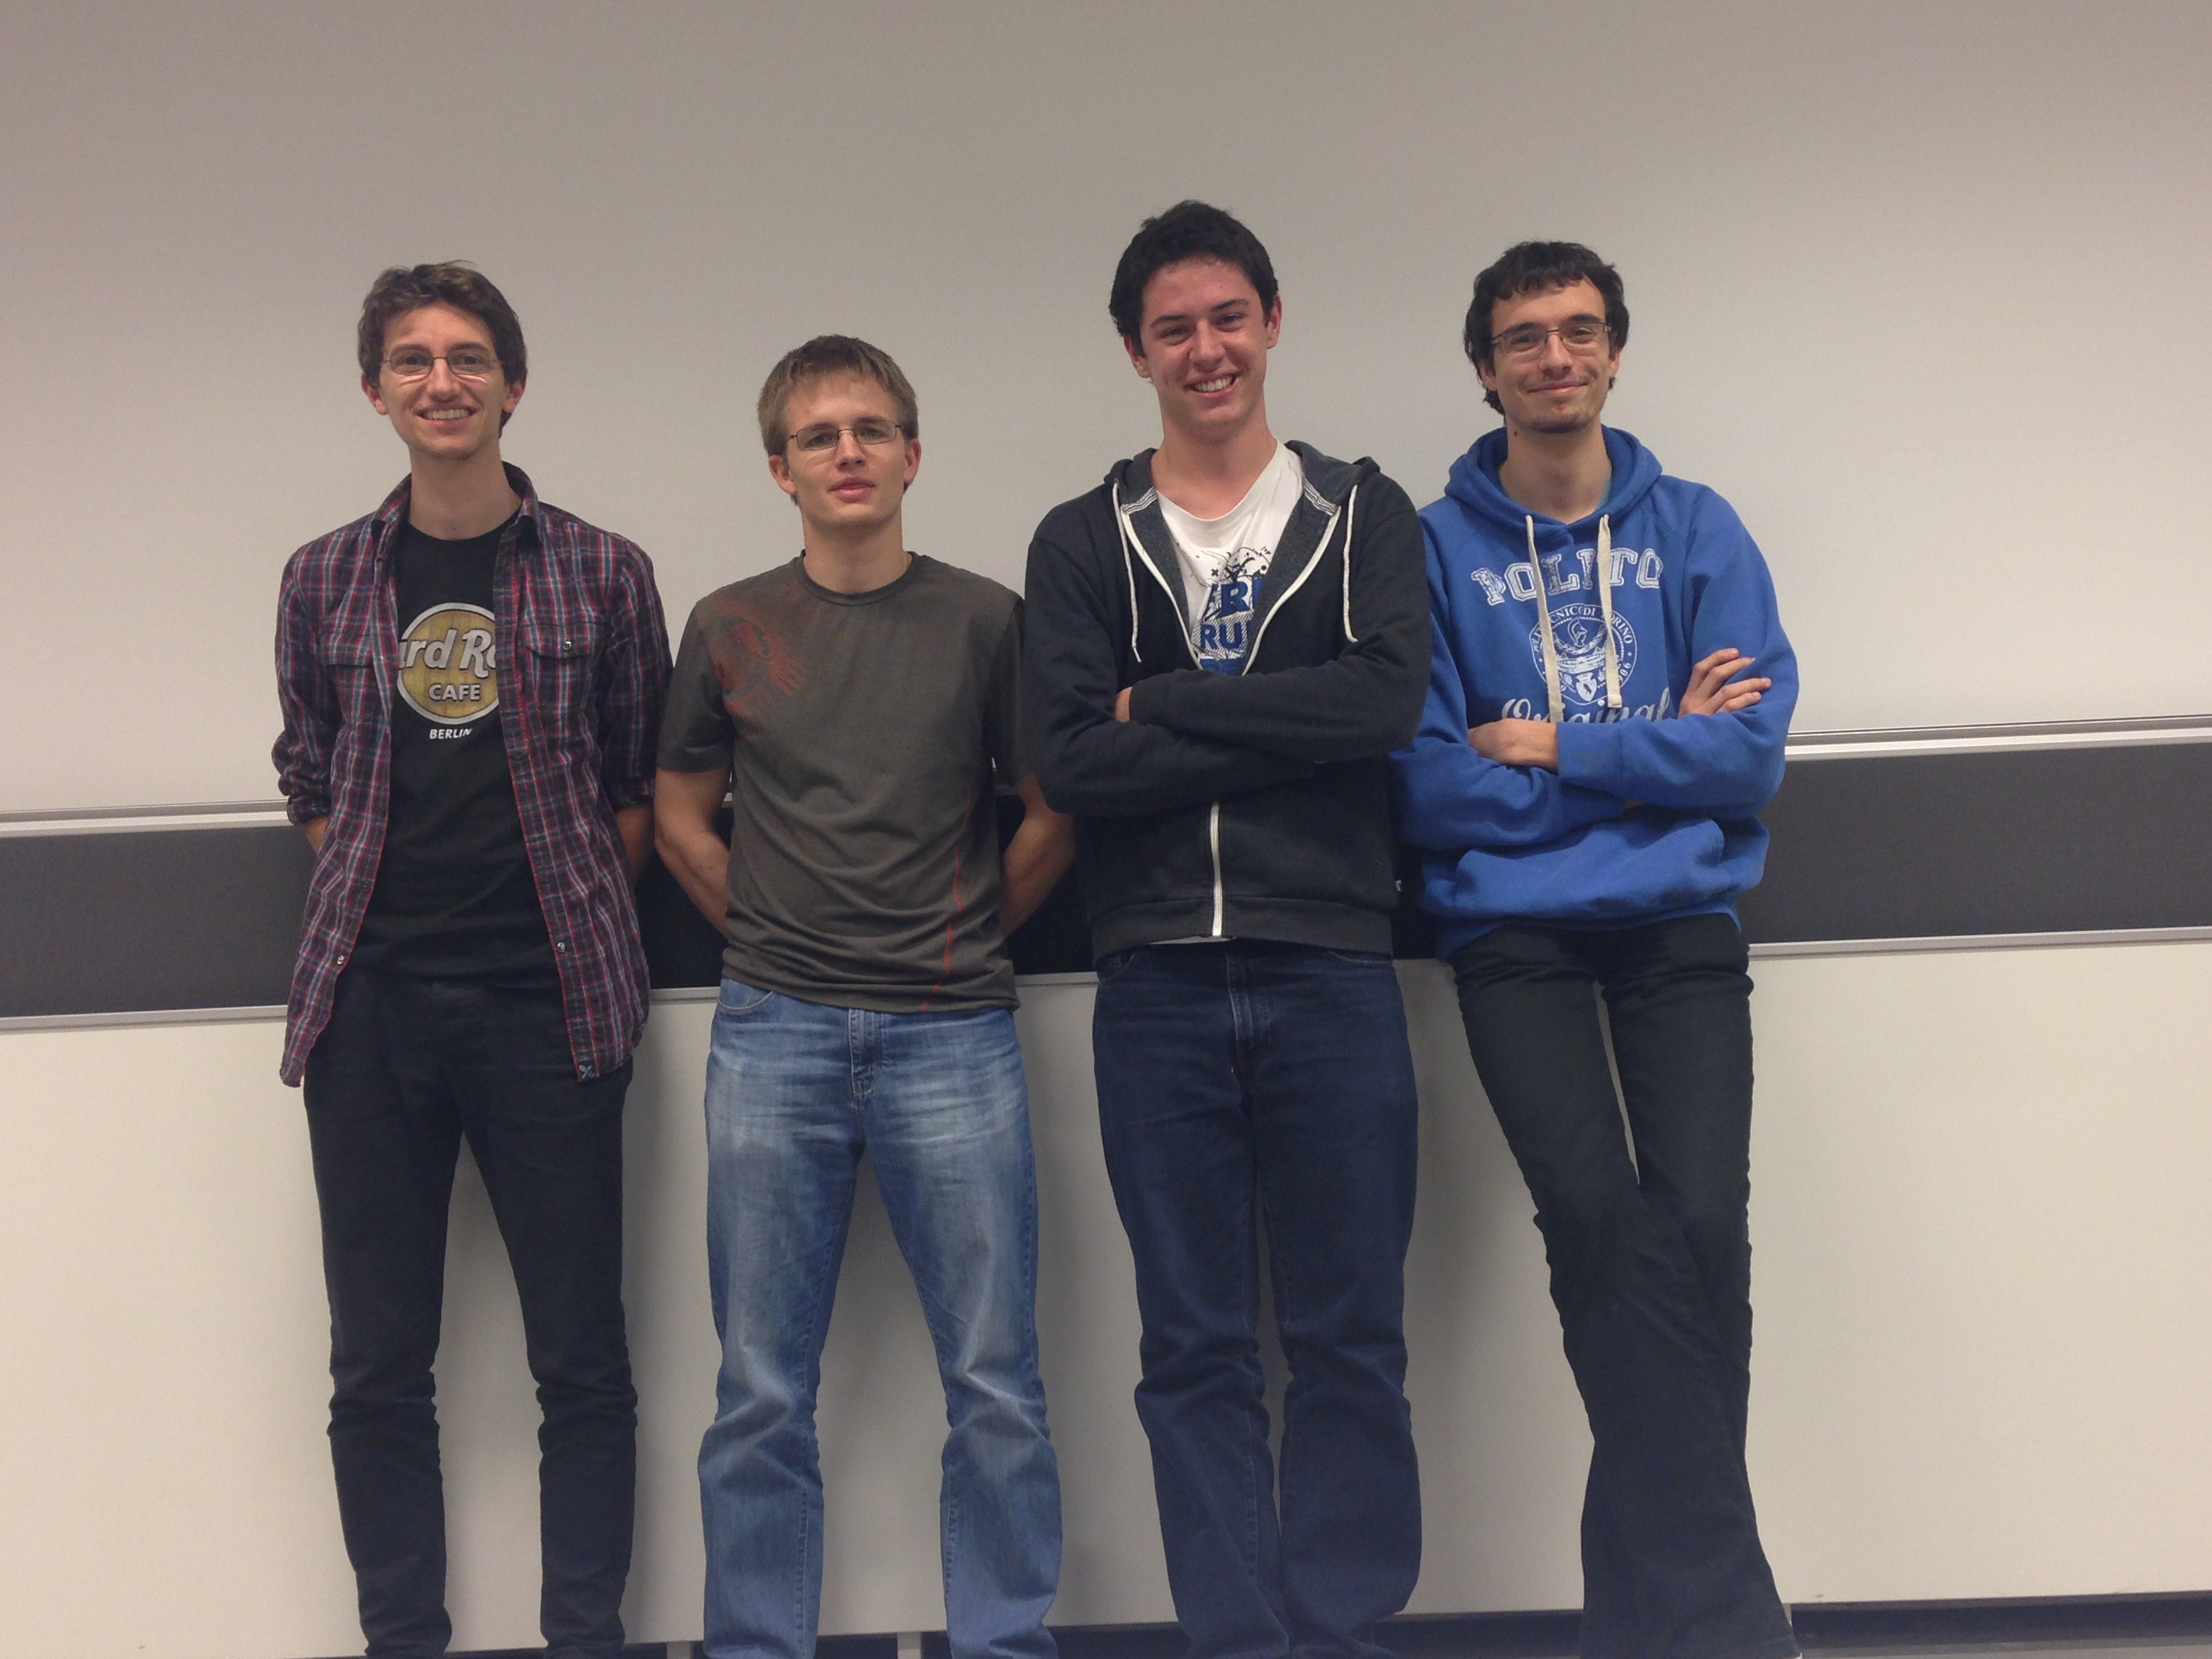
\includegraphics[height=4cm]{portrait.jpg}
\end{figure}
\end{frame}

\begin{frame}
\frametitle{Sommaire}
\tableofcontents
\end{frame}

%Sujet abord�
%Enjeux soci�taux identifi�s
%Motivations personnelles
%Th�se et hypoth�ses
%Propres adh�sions/convictions pour th�se/hypoth�ses (de 1 � 6)

\begin{frame}
\section{Google Glass}
\frametitle{Google Glass}
\begin{columns}
    \begin{column}{0.48\textwidth}
       	\begin{itemize}
		\item Cam�ra int�gr�e
		\item Micro
		\item Pav� tactile
		\item Mini �cran
		\item Acc�s internet
		\item Ecouteur
		\end{itemize}
    \end{column}
    \begin{column}{0.48\textwidth}
		\begin{figure}
		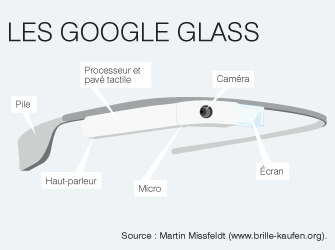
\includegraphics[height=4cm]{glass.jpg}
		\end{figure}
    \end{column}
\end{columns}

Acc�s � toutes les fonctionnalit�s de google, similaire a un smartphone
\end{frame}


\begin{frame}
\section{Enjeux soci�taux}
\frametitle{Enjeux soci�taux}
\begin{itemize}
\item Respect de la vie priv�e
\item Interactions sociales
	\begin{enumerate}
	\item Politesse
	\item D�sinvestissement
	\item D�pendance � la technologie
	\end{enumerate}
\item 
\end{itemize}
\end{frame}


\begin{frame}
\section{Motivation personnelles}
\frametitle{Motivation personnelles}
\begin{itemize}
\item Curiosit� par rapport aux nouvelles technologies
\item Eventail de possibilit�s offertes par les Google Glass
\item Comprendre pourquoi une technologie attractive, qui fonctionne engendre autant de pol�miques et n'est pas commercialis�e (pour l'instant)
\end{itemize}
\end{frame}


\begin{frame}
\section{Probl�matique}
\frametitle{Probl�matique}
Comment l....
\end{frame}

\begin{frame}
\section{Th�se et hypoth�ses}
\frametitle{Th�se et hypoth�ses}
\end{frame}

\begin{frame}
\section{Propres adh�sions/convictions}
\frametitle{Propres adh�sions/convictions}
\end{frame}




\end{document}